\section{Camera Translation Tracking}
\label{Sec:CamTransTrackExp}

Experiments measuring the difference between the ground-truth camera movement and the registered camera movement using the FVR method are presented in this section. For these experiments, one camera frame of an office environment was captured using the ASUS Xtion PRO LIVE active camera. The camera was then moved (translated) by different amounts including: 5 centimeters, 10 centimeters and 15 centimeters. These distances were measured using a measuring tool, and a second frame was then captured. The FVR method was used to register both frames in order to measure the camera location separation between the frames. \\

Different levels of noise were added to both frames prior to 3D registration in order to measure the FVR registration method's ability to register frames with large amounts of noise. The Signal to Noise Ratio (SNR) metric is used to describe the noise added to both captured frames, prior to any registration. This noise effects any registration method's ability to accurately estimate the transformation separating two sets of data. A noise range value of $x$\% means random noise was added in the range [$\frac{-x}{2}$, $\frac{x}{2}$]. Camera registration error is measured in both centimetres (cm) and voxel error (the error in the phase correlation volume without taking into account the effects of quantization). Table \ref{table:trans} shows the results of these tests, they illustrate the FVR's robustness to noise whilst registering frames which are captured during different camera translation intervals. \\

%translation
\begin{table}[!htb]
\centering
\scalebox{1.0}{
\begin{tabular}{cccccccc}
\\ \textbf{10deg} &   &   &   &   &   &   &   \\ 
 & \textbf{FM2D} & \textbf{FM3D} & \textbf{ICP} & \textbf{PCA} & \textbf{FVR} & \textbf{FFVR} & \textbf{FVR3D} \\ \hline
0 &  0.17 & 9.77 & 0.19 & 0.3 & 0.18 & 0.35 & 4.05 \\
0.1 &  0.21 & 0.41 & 0.17 & 0.67 & 0.15 & 0.21 & 10.54 \\
0.25 &  0.16 & 0.34 & 0.13 & 0.39 & 0.15 & 0.44 & 5.44 \\
\\ \textbf{20deg} &   &   &   &   &   &   &   \\ 
 & \textbf{FM2D} & \textbf{FM3D} & \textbf{ICP} & \textbf{PCA} & \textbf{FVR} & \textbf{FFVR} & \textbf{FVR3D} \\ \hline
0 &  1.37 & 13.1 & 1.81 & 16.93 & 7.29 & 1.32 & 3.18 \\
0.1 &  1.35 & 14.32 & 15.29 & 2.97 & 36611.7 & 2.03 & 1.92 \\
0.25 &  1.6 & 3.26 & 14.7 & 0.64 & 1.54 & 4.29 & 2.24 \\
\\ \textbf{30deg} &   &   &   &   &   &   &   \\ 
 & \textbf{FM2D} & \textbf{FM3D} & \textbf{ICP} & \textbf{PCA} & \textbf{FVR} & \textbf{FFVR} & \textbf{FVR3D} \\ \hline
0 &  3.87 & 10.15 & 3.16 & 9.97 & 2.11 & 5.68 & 3.63 \\
0.1 &  3.77 & 16.65 & 39.37 & 77.6 & 4.45 & 2.82 & 1.39 \\
0.25 &  3.68 & 2.76 & 5.12 & 5.78 & 3.3 & 7.15 & 6.38 \\
\\
\end{tabular}}
\\
\caption{Translation Tracking}
\label{table:trans}
\end{table}

%translation
\begin{table}[!htb]
\centering
\scalebox{1.0}{
\begin{tabular}{cccccccc}
\\ \textbf{5cm} &   &   &   &   &   &   &   \\ 
 & \textbf{FM2D} & \textbf{FM3D} & \textbf{ICP} & \textbf{PCA} & \textbf{FVR} & \textbf{FFVR} & \textbf{FVR3D} \\ \hline
0 &  5.07 & 4.75 & 12.35 & 3.73 & 4.04 & fail & 6.24 \\
0.1 &  18.96 & fail & fail & 2.33 & 2.73 & 14.6 & 5.63 \\
0.25 &  5.12 & 4.3 & 2.03 & 4.2 & 4.13 & 5.51 & 2.3 \\
0.5 &  5.61 & 1.95 & 3.71 & 6.83 & 3.7 & 7.73 & 2.83 \\
0.7 &  5.02 & 8.57 & 6.41 & 20.94 & 2.24 & 6.5 & 4.33 \\
\\ \textbf{10cm} &   &   &   &   &   &   &   \\ 
 & \textbf{FM2D} & \textbf{FM3D} & \textbf{ICP} & \textbf{PCA} & \textbf{FVR} & \textbf{FFVR} & \textbf{FVR3D} \\ \hline
0 &  15.35 & fail & 10.26 & 16.87 & 3.47 & fail & 7.07 \\
0.1 &  18.2 & 15.36 & 6.24 & fail & 3.89 & fail & 11.45 \\
0.25 &  fail & 24.12 & 6.02 & 20.12 & 5.4 & fail & 7.53 \\
0.5 &  fail & 4.42 & 5 & 3.96 & 4.65 & fail & 9.47 \\
0.7 &  7.27 & 8.57 & 3.98 & 7.85 & 15.45 & fail & 4.3 \\
\\ \textbf{15cm} &   &   &   &   &   &   &   \\ 
 & \textbf{FM2D} & \textbf{FM3D} & \textbf{ICP} & \textbf{PCA} & \textbf{FVR} & \textbf{FFVR} & \textbf{FVR3D} \\ \hline
0 &  fail & fail & 7.85 & fail & 25.87 & fail & fail \\
0.1 &  fail & fail & 7.13 & fail & 12.27 & fail & fail \\
0.25 &  15.17 & fail & fail & fail & 8.1 & 12.52 & fail \\
0.5 &  fail & fail & 11.11 & fail & 10.13 & 11.09 & fail \\
0.7 &  fail & fail & 10.31 & 20.59 & 7.79 & fail & fail \\
\\
\end{tabular}}
\\
\caption{Translation Tracking}
\label{table:trans}
\end{table}



%translation
\begin{table}[!htb]
\centering
\scalebox{1.0}{
\begin{tabular}{cccccccc}
\\ \textbf{10deg} &   &   &   &   &   &   &   \\ 
 & \textbf{FM2D} & \textbf{FM3D} & \textbf{ICP} & \textbf{PCA} & \textbf{FVR} & \textbf{FFVR} & \textbf{FVR3D} \\ \hline
0 &  1.86 & 1304.46 & 1.18 & 1.35 & 1.01 & 1.18 & 6.75 \\
0.1 &  2.52 & 1.36 & 1.1 & 1.09 & 1.03 & 1.47 & 1.79 \\
0.25 &  11.47 & 0.99 & 1 & 1.22 & 1.07 & 1.1 & 7.37 \\
0.5 &  1.92 & 11.74 & 1.01 & 1.03 & 0.97 & 1.45 & 6.76 \\
0.75 &  46.55 & 1.04 & 1.26 & 1.41 & 3.13 & 1.53 & 4.94 \\
\\ \textbf{20deg} &   &   &   &   &   &   &   \\ 
 & \textbf{FM2D} & \textbf{FM3D} & \textbf{ICP} & \textbf{PCA} & \textbf{FVR} & \textbf{FFVR} & \textbf{FVR3D} \\ \hline
0 &  142.17 & 14 & 5.31 & 3.82 & 4.45 & 8.16 & 35.15 \\
0.1 &  6.98 & 110.77 & 4.65 & 6.87 & 5.71 & 4.93 & 9.77 \\
0.25 &  19.73 & 551.95 & 4.4 & 15.7 & 53.85 & 43.63 & 8.31 \\
0.5 &  6.2 & 590.04 & 5.31 & 3.48 & 5.28 & 6.46 & 25.57 \\
0.75 &  8.67 & 18.53 & 5.78 & 4.89 & 8.38 & 7.08 & 8.61 \\
\\ \textbf{30deg} &   &   &   &   &   &   &   \\ 
 & \textbf{FM2D} & \textbf{FM3D} & \textbf{ICP} & \textbf{PCA} & \textbf{FVR} & \textbf{FFVR} & \textbf{FVR3D} \\ \hline
0 &  242.6 & 11.64 & 5.62 & 160.32 & 4.37 & 31.39 & 159.64 \\
0.1 &  24.22 & 9.7 & 4.73 & 115.38 & 25.33 & 18.36 & 28.11 \\
0.25 &  35.76 & 15.01 & 3 & 138.62 & 8.05 & 17.78 & 21.09 \\
0.5 &  48.64 & 34.73 & 3.03 & 22.81 & 7.71 & 9.33 & 37.75 \\
0.75 &  23.63 & 63.56 & 3.53 & 72.88 & 10.86 & 23.71 & 21.51 \\
\\
\end{tabular}}
\\
\caption{Translation Tracking}
\label{table:trans}
\end{table}

   
%translation
\begin{table}[!htb]
\centering
\scalebox{1.0}{
\begin{tabular}{ccccc}
\hline
\textbf{translation (cm)} & \textbf{noise range (\%)} & \textbf{SNR} & \textbf{error (cm)} & \textbf{error (voxel)}\\ \hline
5cm & 0 & $\infty$ & 0 & 0\\
5cm & 10 & 20db & 0 & 0\\
5cm & 25 & 12db & 0 & 0\\
5cm & 50 & 6db & 0 & 0\\
5cm & 75 & 2.5db & 112.28 & 89.83\\
10cm & 0 & $\infty$ & 0 & 0\\
10cm & 10 & 20db & 0 & 0\\
10cm & 25 & 12db & 0 & 0\\
10cm & 50 & 6db & 156.65 & 125.32\\
15cm & 0 & $\infty$ & 2.8 & 2.24\\
15cm & 10 & 20db & 2.8 & 2.24\\
15cm & 25 & 12db & 2.8 & 2.24\\
15cm & 50 & 6db & 198.55 & 158.84\\
\\
\end{tabular}}
\\
\caption{Translation Tracking}
\label{table:trans}
\end{table}

Results show that the FVR method is accurately able to register frames up to 15 centimeters apart and for camera movements below 5 centimeters per frame, the FVR method can accurately register them. Results also indicate that, for these camera movements the FVR method can handle up to 75\% noise within the frame, which is a Signal to Noise (SNR) ratio of as little as 2.5 decibels. \\

It can be shown that the registration of camera movements using the FVR can handle movements up to 15cm as long as the SNR is higher than or equal to 6.0, meaning the FVR method is highly robust to noise. To put these camera translations into perspective at video frame rates, a displacement of 10 centimeters per frame equates to camera velocity of 3 meters per second which is about twice the normal walking speed. This is suitable for a majority of applications. \\


\section{Camera Rotation Tracking}
\label{Sec:CamRoteTrackExp}

Table \ref{table:rote} shows results for camera rotation experiments. The experiments, also captured with the ASUS Xtion PRO LIVE active camera, were created by capturing the first frame befroe rotating the camera about the y-axis by a number of degrees. The degrees were measured between rotations. Degrees of separation tested include: 10, 20 and 30 degrees. \\

Again, different levels of noise were added to both frames prior to registration. This experiment was designed to test the robustness of the FVR method in registering camera pose. The scene captured was the same office environment used in the translation experiment from section \ref{Sec:CamTransTrackExp}. \\

\begin{table}[!htb]
\centering
\scalebox{1.0}{
\begin{tabular}{ccccc}
\hline
\textbf{rotation} & \textbf{noise (\%)} & \textbf{SNR} & \textbf{error ($\theta$)} & \textbf{error (voxel)}\\ \hline
$10^{\circ}$ & 0 & $\infty$ & 0.31 & 0\\
$10^{\circ}$ & 10 & 20db & 0.31 & 0\\
$10^{\circ}$ & 25 & 12db & 0.63 & 1\\
$10^{\circ}$ & 30 & 10.5db & 90.62 & 96\\
$20^{\circ}$ & 0 & $\infty$ & 0.31 & 0\\
$20^{\circ}$ & 10 & 20db & 0.63 & 1\\
$20^{\circ}$ & 15 & 16.5db & 38.13 & 40\\
$30^{\circ}$ & 0 & $\infty$ & 3.75 & 4\\
$30^{\circ}$ & 10 & 20db & 3.28 & 3\\
$30^{\circ}$ & 15 & 16.5db & 30 & 32\\
\\
\end{tabular}}
\\
\caption{Rotation Tracking}
\label{table:rote}
\end{table}

Twelve degrees per frame is almost a full rotation per second in video rates. This is so fast that most cameras would acquire too much motion blur for registration to be possible. Therefore this test indicates the robustness of the FVR method within the context of camera pose estimation. \\

Given 10 degrees of separation, the error was below 1 degree for noise levels less than or equal to 30\%. This base line error is due to the sampling resolution of the volume, as voxel error was in fact zero. This metric removes the error which is primarily due to quantization noise. As with the translation experiments, the effect of noise increases with camera disparity. At 30 degrees of camera rotation, little matching information is available in order to perform a registration for most techniques. However, for noise levels of 10\% or less, voxel distance error was as low as 4 with an angular error less than $3.8$ degrees. As mentioned, rotations of this magnitude are unlikely as motion blur would occur. Therefore these results show both the effectiveness of the FVR in terms of pose registration, as well as robustness to noise interference. \\


\section{Object Motion Experiments}
\label{Sec:FVRMotionExp}

\begin{table}[!htb]
\centering
\scalebox{1.0}{
\begin{tabular}{ccc}
\hline
\textbf{Object Size} & \textbf{error (cm)} & \textbf{error (voxel)}\\ \hline
0.35 & 0 & 0\\
2.95 & 0 & 0\\
6.22 & 0 & 0\\
12.28 & 0 & 0\\
19.82 & 0 & 0\\
22.39 & 0 & 0\\
26.09 & 0 & 0\\
31.00 & 0 & 0\\
48.23 & 38.42 & 15\\
74.32 & 113.57 & 44\\
\\
\end{tabular}}
\\
\caption{Object Motion Test}
\label{table:OBJECT_MOVE_EXP}
\end{table}


In order to assess robustness to object motion, experiments were conducted by moving the ASUS Xtion PRO LIVE active camera backwards along the z-axis by 5 centimeters per frame whilst moving objects were placed in and out of the scene so that they only appear in one of the volumes being registered. Various sized objects including stacks of CDs, large boxes, people and several pieces of furniture were used and are measured by the percentage of the frame they occupy. Results from table \ref{table:OBJECT_MOVE_EXP} show the proposed method was accurate upto an object size of 31\%, but failed for objects taking up over 48.23\%.

\section{Reconstructed Scenes}
\label{Sec:FVRQual1Exp}

\begin{figure}[!htb] 
        \centering
        \begin{subfigure}[b]{3.0in}
                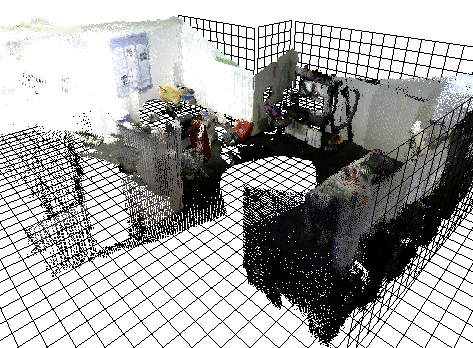
\includegraphics[width=3.0in]{images/ch2/unit21}
                \caption{Apartment}
                \label{fig:RECON_UNIT}
        \end{subfigure}
        \begin{subfigure}[b]{3.0in}
                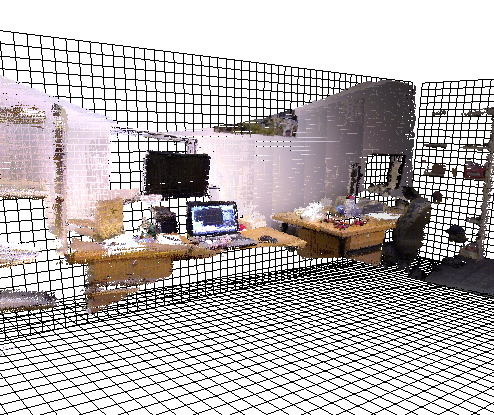
\includegraphics[width=3.0in]{images/ch2/officeA}
                \caption{Office}
                \label{fig:RECON_OFFICE}
        \end{subfigure}
        \begin{subfigure}[b]{3.0in}
                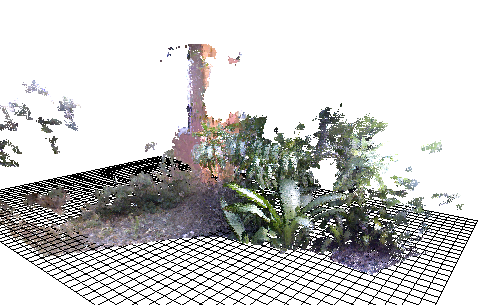
\includegraphics[width=3.0in]{images/ch2/outdoorA}
                \caption{Garden}
                \label{fig:RECON_GARDEN}
        \end{subfigure}
       \caption{Reconstructed Scenes.}
       \label{fig:RECONSTRUCTIONS}
\end{figure}

Qualitative experiments also show the ability of the FVR registration method to reconstruct 3D scenes. In these experiments, two indoor environments (Apartment and Office) as well as one outdoor environment (Garden) were reconstructed and are shown in figures \ref{fig:RECON_UNIT}, \ref{fig:RECON_OFFICE} and \ref{fig:RECON_GARDEN} respectively. \\

The Apartment reconstruction was recorded by moving the ASUS Xtion PRO LIVE active camera through a room and rotating the camera. Each frame was registered using the FVR algorithm. Some of the frames in the apartment scene contain walls which have few features. Between frames, walls also had colour contrast shifts. These shifts are due to the ASUS camera's automatic contrast feature which adjusts contrast based on colour histograms. Despite these setbacks, accurate 3D reconstruction was achieved by the FVR method as illustrated in figure \ref{fig:RECON_UNIT}. \\


The office reconstruction was also generated by rotating the ASUS Xtion PRO LIVE active camera about the y-axis while moving the camera around the room. This time, during rotation, the camera was focused on both foreground and background objects. Here, the entire video sequence was accurately registered. It can be seen that despite the foreground and background focus, the global reconstruction is accurate. This scene, as in the apartment scene has usable texture which should not cause large amounts of texture confusion. These qualitative experiments show that despite being a closed form solution, the FVR has reconstruction accuracy comparable to existing feature based SLAM methods. \\


Typical feature based methods work well with indoor environments where local features are readily distinguishable and easy to match. They do not tend to work as well in complex outdoor scenes where feature confusion is likely. To assess performance in such outdoor scenes, a garden scene containing bushes, plants and a ground covering of bark and rocks was captured for testing. Again, this scene was captured using the ASUS Xtion PRO LIVE active camera moving around the out-door garden. The proposed FVR method was able to produce a good quality reconstruction of this garden scene, as shown in figure \ref{fig:RECON_GARDEN}. This shows that reconstruction approaches which integrate or make use of the FVR registration method may have an advantage in performing 3D reconstructions in these types of scenes, scenes which are of common disturbance to many existing feature matching methods, as expressed in the literature.   

